%%%%%%%%%%%%%%%%%%%%%%%%%%%%%%%%%%%%%%%%%
% Short Sectioned Assignment
% LaTeX Template
% Version 1.0 (5/5/12)
%
% This template has been downloaded from:
% http://www.LaTeXTemplates.com
%
% Original author:
% Frits Wenneker (http://www.howtotex.com)
%
% License:
% CC BY-NC-SA 3.0 (http://creativecommons.org/licenses/by-nc-sa/3.0/)
%
%%%%%%%%%%%%%%%%%%%%%%%%%%%%%%%%%%%%%%%%%

%----------------------------------------------------------------------------------------
%	PACKAGES AND OTHER DOCUMENT CONFIGURATIONS
%----------------------------------------------------------------------------------------

% !TeX spellcheck = es_ES
\documentclass[paper=a4, fontsize=11pt]{scrreprt} % A4 paper and 11pt font size

\usepackage[spanish]{babel}
\usepackage[utf8]{inputenc}

\usepackage[T1]{fontenc} % Use 8-bit encoding that has 256 glyphs
\usepackage{fourier} % Use the Adobe Utopia font for the document - comment this line to return to the LaTeX default

\usepackage{amsmath,amsfonts,amsthm} % Math packages
\usepackage{sectsty} % Allows customizing section commands

\usepackage[pdftex]{graphicx}

\usepackage{listings}

\usepackage{calc}

\usepackage{appendix}

\newlength{\imgwidth}

\newcommand\scalegraphics[1]{
    \settowidth{\imgwidth}{\includegraphics{#1}}
    \setlength{\imgwidth}{\minof{\imgwidth}{\textwidth}}
    \includegraphics[width=\imgwidth]{#1}
}

\allsectionsfont{\centering \normalfont\scshape} % Make all sections centered, the default font and small caps
\usepackage{float}
\usepackage{fancyhdr} % Custom headers and footers
\pagestyle{fancy} % Makes all pages in the document conform to the custom headers and footers
\fancyhead{} % No page header - if you want one, create it in the same way as the footers below
\fancyfoot[L]{} % Empty left footer
\fancyfoot[C]{} % Empty center footer
\fancyfoot[R]{\thepage} % Page numbering for right footer
\renewcommand{\headrulewidth}{0pt} % Remove header underlines
\renewcommand{\footrulewidth}{0pt} % Remove footer underlines
\setlength{\headheight}{13.6pt} % Customize the height of the header

\numberwithin{equation}{section} % Number equations within sections (i.e. 1.1, 1.2, 2.1, 2.2 instead of 1, 2, 3, 4)
\numberwithin{figure}{section} % Number figures within sections (i.e. 1.1, 1.2, 2.1, 2.2 instead of 1, 2, 3, 4)
\numberwithin{table}{section} % Number tables within sections (i.e. 1.1, 1.2, 2.1, 2.2 instead of 1, 2, 3, 4)

\setlength\parindent{0pt} % Removes all indentation from paragraphs - comment this line for an assignment with lots of text

\def\ScaleIfNeeded{
    \ifdim\Gin@nat@width>\linewidth
    \linewidth
    \else
    \Gin@nat@width
    \fi
}


\usepackage[usenames,dvipsnames]{color}
% This is the color used for MATLAB comments below
\definecolor{MyDarkGreen}{rgb}{0.0,0.4,0.0}

% For faster processing, load Matlab syntax for listings
\lstloadlanguages{Matlab}
\lstset{language=Matlab,                        % Use MATLAB
    columns=fullflexible,
    frame=single,                           % Single frame around code
    basicstyle=\tiny\ttfamily,             % Use small true type font
    keywordstyle=[1]\color{Blue}\bf,        % MATLAB functions bold and blue
    keywordstyle=[2]\color{Purple},         % MATLAB function arguments purple
    keywordstyle=[3]\color{Blue}\underbar,  % User functions underlined and blue
    identifierstyle=,                       % Nothing special about identifiers
    % Comments small dark green courier
    commentstyle=\usefont{T1}{pcr}{m}{sl}\color{MyDarkGreen}\small,
    stringstyle=\color{Purple},             % Strings are purple
    showstringspaces=false,                 % Don't put marks in string spaces
    tabsize=5,                              % 5 spaces per tab
    %
    %%% Put standard MATLAB functions not included in the default
    %%% language here
    morekeywords={xlim,ylim,var,alpha,factorial,poissrnd,normpdf,normcdf},
    %
    %%% Put MATLAB function parameters here
    morekeywords=[2]{on, off, interp},
    %
    %%% Put user defined functions here
    morekeywords=[3]{},
    %
    morecomment=[l][\color{Blue}]{...},     % Line continuation (...) like blue comment
    numbers=left,                           % Line numbers on left
    firstnumber=1,                          % Line numbers start with line 1
    numberstyle=\tiny\color{Blue},          % Line numbers are blue
    stepnumber=1                            % Line numbers go in steps of 5
}

%----------------------------------------------------------------------------------------
%	TITLE SECTION
%----------------------------------------------------------------------------------------

\newcommand{\horrule}[1]{\rule{\linewidth}{#1}} % Create horizontal rule command with 1 argument of height

\title{
    \normalfont \normalsize 
    \textsc{Robótica Industrial} \\ [25pt] % Your university, school and/or department name(s)
    \horrule{0.5pt} \\[0.4cm] % Thin top horizontal rule
    \huge Práctica 5: Robot Real \\ % The assignment title
    \horrule{2pt} \\[0.5cm] % Thick bottom horizontal rule
}

\author{Juan Antonio Aldea Armenteros} % Your name

\date{\normalsize\today} % Today's date or a custom date

\begin{document}

    \maketitle % Print the title
    \chapter{Intento de control manual}
    Realmente no hay mucho que decir, estuve intentando manejar el robot de forma manual pero este se mostró reticente, el tiempo de respuesta era bastante largo en la mayoría de ocasiones y en bregar con eso se perdió toda la sesión, de el método de control programático parecía funcionar correctamente pero la sesión terminó sin realizar ninguna prueba digna de mención. Fue bastante frustrante.
    \newline
    \begin{figure}[H]
        \centering
        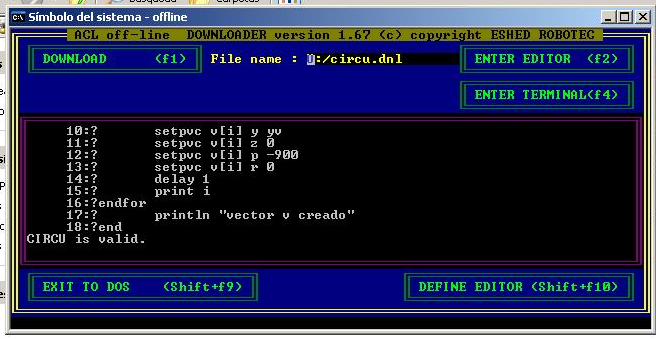
\includegraphics[width=15cm]{imagenes/entorno_programacion.png}
        \caption{Captura del entorno de programación.}
    \end{figure}
    \chapter{Intento de trayectoria circular}
    Abandoné el robot de la sesión anterior y me puse con un compañero, intentamos programar la trayectoria circular usando la forma paramétrica de la ecuación de la circunferencia, esto sirvió para descubrir algunas curiosas características del lenguaje ACL, es poco más que un ensamblador con (aparente) ausencia total de ortogonalidad (la  ortogonalidad de un lenguaje es una propiedad de coherencia y homogeneidad semántica y estructural), cosas como \lstinline{X = FACTOR * COS VARIABLE} siendo FACTOR obligatorio en la sentencia son un buen ejemplo de lo que comento.
    \newline
    Volviendo al contenido de la práctica, compilamos y probamos el código que se da como ejemplo en la documentación de la práctica la trayectoria en forma de U, funcionó sin grandes problemas (grabé un video con el móvil pero dado que aparecen algunas caras y no he conseguido emborronarlas, he preferido no subirlo a YouTube). Después sustituimos el calculo de los puntos por las funciones paramétricas de la circunferencia pero no logramos que funcionara correctamente ya que siempre devolvia "bad coordinate" (o mensaje similar), error debido a algún problema a la hora de la generación de la trayectoria, coordenadas inalcanzables, desplazamiento demasiado pequeño o quién sabe qué. Como curiosidad otro compañero que estaba usando el mismo robot no tenía problemas usando el 0 valor de Y para las coordenadas del circulo, sin embargo en nuestro robot eso era motivo del ya mencionado mensaje "bad coordinate".
    \newline
    \lstinputlisting[caption = Código para generar los puntos de una trayectoria circular]{codigos/circu.dnl}
\end{document}